\chapter{Homological algebra}\label{chapter:hom_alg}

    References for this chapter are \cite{weibel,hom_algebra}.

\section{Chain complexes}

	\newdef{Chain complex}{\index{chain!complex}\index{boundary}\index{differential}\index{cycle}\index{exact!element}\index{closed!element}\label{homalg:chain_complex}
		\nomenclature[S_CH]{$C_\bullet$}{chain complex}
		\nomenclature[S_CHCat]{$\textbf{Ch}(\textbf{A})$}{category of chain complexes with objects in the additive category $\textbf{A}$}
		Let $\mathbf{A}$ be an additive category (often an Abelian category) and consider a collection $\{C_k\}_{k\in\mathbb{Z}}$ of objects and a collection $\{\partial_k:C_k\rightarrow C_{k-1}\}_{k\in\mathbb{Z}}$ of morphisms in $\mathbf{A}$ such that for all $k\in\mathbb{Z}$:
		\begin{gather}
			\partial_k\circ\partial_{k+1} = 0.
		\end{gather}
		This structure is called a chain complex\footnote{A \textbf{cochain complex} is constructed similarly with an ascending order $\partial_k:C_k\rightarrow C_{k+1}$.} and the morphisms $\partial_k$ are called the \textbf{boundary operators} or \textbf{differentials}. Elements of $\im(\partial_k)$ are called \textbf{boundaries} or \textbf{exact elements} and elements of $\ker(\partial_k)$ are called \textbf{cycles} or \textbf{closed elements}. The chain complex $\{(C_k,\partial_k)\}_{k\in\mathbb{Z}}$ is often denoted by $(C_\bullet,\partial_\bullet)$ or simply by $C_\bullet$ if the choice of boundary operators is clear.
	}

	Morphisms between chain complexes are called \textbf{chain maps} and they are defined as collections of morphisms $\{f_k:C_k\rightarrow D_k\}_{k\in\mathbb{Z}}$ such that for all $k\in\mathbb{Z}$ the following equation holds:
	\begin{gather}
		\partial'_k\circ f_k = f_{k-1}\circ\partial_k\,,
	\end{gather}
	where $\partial_k,\partial_k'$ are the boundary operators of $C_\bullet$ and $D_\bullet$, respectively. Given an additive category $\mathbf{A}$, one writes $\mathbf{Ch}(\mathbf{A})$ for the category of chain complexes and chain maps in $\mathbf{A}$.

	\begin{remark}[Reversal]
        Given a chain (resp.~cochain) complex $C$ one can easily construct a cochain (resp.~chain) complex $\widetilde{C}$ by setting $\widetilde{C}_k := C_{-k}$.
    \end{remark}

	\newdef{Chain homology}{\index{homology}\label{homalg:homology}
		Given a chain complex $C_\bullet$, one can define a sequence of \textbf{homology groups} $H_n(C_\bullet)$. Since $\partial^2=0$, the kernel $\ker(\partial_k)$ is a subgroup of the image $\im(\partial_{k+1})$ and it is even a normal subgroup. This way one can define the quotient group:
		\begin{gather}
			H_k(C_\bullet) := \frac{\ker(\partial_k)}{\im(\partial_{k+1})}.
		\end{gather}
		The kernel in this definition, the group of $k$\textbf{-cycles}, is denoted by $Z_k(C_\bullet)$. The image, the group of $(k+1)$\textbf{-boundaries}, is denoted by $B_k(C_\bullet)$. The homology groups themselves also form a chain complex $H_\bullet(C_\bullet)$, but with trivial differentials.
	}

	\newdef{Quasi-isomorphism}{\index{quasi-!isomorphism}
		A chain map for which the induced morphisms on homology are isomorphisms.
	}

	\newdef{Chain homotopy}{\index{chain!homotopy}
		Two chain maps $f,g: C_\bullet\rightarrow D_\bullet$ are said to be chain-homotopic if there exists a chain map $s:C_\bullet\rightarrow D_\bullet$ such that the following equation is satisfied:
		\begin{gather}
			f-g = s\circ\partial_C + \partial_D\circ s.
		\end{gather}
        A chain map that is homotopy-equivalent to the zero map is said to be \textbf{null-homotopic}. If there exist two chain maps $f:C_\bullet\leftrightarrows D_\bullet:g$ such that both $f\circ g$ and $g\circ f$ are chain-homotopic to the identity, $C_\bullet$ and $D_\bullet$ are said to be \textbf{(chain-)homotopy equivalent}.
	}

	\begin{property}
		Chain-homotopic maps induce coinciding maps in homology. In particular, every (chain-)homotopy equivalence is a quasi-isomorphism.
	\end{property}
    \begin{result}[Vanishing homology]\label{homalg:null_acyclic}
        If a null-homotopic chain map $f:C_\bullet\rightarrow C_\bullet$ exists, then $H_\bullet(C_\bullet)$ vanishes.
    \end{result}

    \newdef{Differential modulo differential}{\label{homalg:differential_modulus_differential}
        Consider a chain complex $(C_\bullet,\partial_\bullet)$ together with a chain endomorphism $\dr$. This endomorphism is said to be a differential modulo $\partial$ if it satisfies the following conditions:
        \begin{enumerate}
            \item $\dr\partial+\partial\dr=0$, and
            \item $\dr^2 = [\partial,D]$ for some other chain endomorphism $D$, i.e.~$\dr^2$ is $\partial$-exact in $\End(C_\bullet)$.
        \end{enumerate}
        The first condition states that $\dr$ descends to a chain endomorphism on $H_\bullet(C_\bullet)$. The second condition states that $\dr$ is actually a differential on $H_\bullet(C_\bullet)$. The resulting homology theory is denoted by $H_\bullet(\dr\mid H_\bullet(C_\bullet))$.
    }

    The following definitions use the language of Chapter \ref{chapter:hda}:
    \newdef{Differential graded algebra}{\index{dg-algebra}\label{homalg:dg_algebra}
        \nomenclature[A_DGA]{DGA}{differential graded algebra}
        A differential graded algebra (often called a \textbf{dg-algebra}, \textbf{DGA} or \textbf{dga}) is a (co)chain complex that carries the structure of an algebra where the differential acts as a derivation. Equivalently, it is a graded algebra equipped with a nilpotent derivation of degree $\pm1$.
    }
    \newdef{Connective DGA}{\index{connective}
        A DGA $A_\bullet$ with vanishing (co)homology in negative degree, i.e.~$H_{<0}(A_\bullet)=0$. For every connective DGA, one can find a quasi-isomorphic DGA concentrated in nonnegative degree.
    }
    \newdef{Semifree DGA}{\index{semi-!free}
        A DGA for which the underlying graded algebra is isomorphic (as a graded algebra) to the tensor algebra over a graded vector space.
    }
    \newdef{Differential graded-commutative algebra}{
        \nomenclature[A_DGCA]{DGCA}{differential graded-commutative algebra}
        A graded-commutative differential graded algebra. This is often abbreviated as \textbf{DGCA} or \textbf{dgca}.
    }
    \newdef{Semifree dgca}{
        A DGCA for which the underlying graded-commutative algebra is isomorphic (as a graded-commutative algebra) to the exterior algebra over a graded vector space.
    }

    \newdef{Minimal model}{\index{model}
        Let $(C_\bullet,\partial_\bullet)$ be a (cohomological) DGCA of finite type. A model for $C_\bullet$ is a quasi-isomorphism $\rho:(A_\bullet,\dr_\bullet)\rightarrow(C_\bullet,\partial_\bullet)$ from a semifree DGCA $(A_\bullet,\dr_\bullet)$. This model is said to be \textbf{minimal} if $A_\bullet$ is freely generated in degrees $\geq2$ and satisfies $\dr A\subseteq\Lambda^{\geq2}A$.
    }
    \begin{remark}[\difficult{Model structure on DGCAs}]
        By Property \ref{topology:sullivan_algebras_specific}, the (minimal) models of DGCAs are (minimal) Sullivan algebras. From a model theory point of view, the (minimal) Sullivan algebras are the cofibrant objects and the (minimal) models are the cofibrant replacements.
    \end{remark}

\section{Exact sequences}

	\newdef{Exact sequence}{\index{exact!sequence}
		Let $\mathbf{A}$ be an additive category and consider a sequence of objects and morphisms in $\mathbf{A}$:
		\begin{gather}
			C_0\overset{\Phi_1}{\longrightarrow}C_1\overset{\Phi_2}{\longrightarrow}\cdots\overset{\Phi_n}{\longrightarrow}C_n.
		\end{gather}
		This sequence is said to be exact if for every $k\in\mathbb{N}$:
        \begin{gather}
            \im(\Phi_k) = \ker(\Phi_{k+1}).
        \end{gather}
        In particular this means that $\Phi_{k+1}\circ\Phi_k = 0$ for all $k\in\mathbb{N}$, which in turn implies that exact sequences are a special type of chain complexes \ref{homalg:chain_complex}.
	}
	\newdef{Short exact sequence}{\label{homalg:short_exact_sequence}
		An exact sequence with exactly three nonzero terms:
		\begin{gather}
			0\longrightarrow C_0\overset{\Phi_1}{\longrightarrow}C_1\overset{\Phi_2}{\longrightarrow}C_3\longrightarrow0.
		\end{gather}
		Usually, all other exact sequences are said to be \textbf{long}.
	}

	\begin{property}[Morphisms in exact sequences]
		By looking at some simple examples, one can derive some important constraints for certain exact sequences. Consider the sequence \[0\longrightarrow C\overset{\Phi}{\longrightarrow}D.\] This sequence can only be exact if $\Phi$ is an injective morphism (monomorphism). This follows from the fact that the only element in the image of the map $0\rightarrow C$ is 0 because the map is a morphism. It follows that the kernel of $\Phi$ is trivial and, hence, that $\Phi$ is injective.

		Analogously, the sequence \[C\overset{\Psi}{\longrightarrow}D\longrightarrow0\] is exact if and only if $\Psi$ is a surjective morphism (epimorphism). This follows from the fact that the kernel of the map $D\rightarrow0$ is all of $C$, which implies that $\Psi$ is surjective (by exactness).

		Combining these two cases shows that \[0\longrightarrow C\overset{\Sigma}{\longrightarrow}D\longrightarrow0\] is exact if and only if $\Sigma$ is a \textbf{bimorphism} (if $\mathbf{A}$ is Abelian, $\Sigma$ is even an isomorphism by Property \ref{cat:regular_iso}).
	\end{property}

\section{Resolutions}

	Consider some Abelian category $\mathbf{A}$ and let $\mathbf{Ch(A)}$ denote its category of chain complexes.

	\newdef{Acyclic complex}{\index{acyclic!complex}
		A chain complex $C_\bullet\in\mathbf{Ch}(\mathbf{A})$ is said to be acyclic if the sequence \[\cdots\longrightarrow C_{k+1}\longrightarrow C_k\longrightarrow C_{k-1}\longrightarrow\cdots\] is exact or, equivalently, if the homology complex $H_\bullet(C_\bullet)$ vanishes.
	}
	\sremark{Some references, especially the older ones, use a slightly different definition of acyclicity. In their definition, the sequence is exact except in degree 0, i.e.~$H_0(C_\bullet)\neq0$.}

	\newdef{Resolution}{\index{resolution}\index{augmentation}\label{homalg:resolution}
		Consider an object $X$ in $\mathbf{A}$. A resolution of $X$ is given by an acyclic chain complex in $\mathbf{A}$ of the form
		\begin{gather}
			\cdots\longrightarrow C_1\longrightarrow C_0\overset{\varepsilon}{\longrightarrow} X\longrightarrow 0.
		\end{gather}
        This also implies that $X$ is the zeroth homology group of the chain complex $C_\bullet := \{C_k\}_{k\geq0}$. The morphism $\varepsilon:C_0\rightarrow X$ is often called the \textbf{augmentation map} and the complex $C_\bullet\rightarrow X\rightarrow 0$ is called the \textbf{augmentation} of $C_\bullet$.
	}

	In practice it is often convenient to restrict to a specific type of resolution. For example, by considering chain complexes with only injective or projective objects (Figures \ref{fig:injective_object} and \ref{fig:projective_object}), one obtains injective or projective resolutions. If every object in $A$ admits a projective (resp.~injective) resolution, $\mathbf{A}$ is said to \textbf{have enough projectives} (resp.~\textbf{injectives}).

    \begin{theorem}[Homological perturbation]\label{homalg:homological_perturbation}
        Consider a resolution $(C_\bullet,\partial_\bullet)$ and denote the grading in $C_\bullet$ by $r$, i.e.~$r(x)=k$ whenever $x\in C_k$. Furthermore, consider a differential $d$ modulo $\partial$ of degree 0 and denote the associated grading by $\deg$. There exists a differential $s$ satisfying the following properties:
        \begin{itemize}
            \item $\deg(s) - r(s) = 1$, and
            \item $s = \delta + \dr + \sum_{i=1}^\infty s_{(i)}$, where $r(s_{(i)})=i$ and $\deg(s_{(i)}) = i+1$.
        \end{itemize}
        Moreover, any differential that satisfies these properties has the same homology as $\dr$:
        \begin{gather}
            H_\bullet(s)\cong H_\bullet(\dr\mid H_\bullet(C_\bullet))\equiv H_\bullet(\dr\mid H_0(C_\bullet)).
        \end{gather}
    \end{theorem}

\section{Derived functors}

	Given an additive functor \ref{cat:additive_functor}, one can define its \textbf{prolongation} to the category of chain complexes:
	\newdef{Prolongation}{\index{prolongation}
		Let $\func{F}{A}{A'}$ be an additive functor. The prolongation of $F$ is a functor $\overline{F}:\mathbf{Ch(A)}\rightarrow\mathbf{Ch(A')}$ obtained by applying $F$ to every object in a chain complex and to every diagram in the definition of a chain map. As is common, by abuse of notation the prolongation will also often be denoted by $F$.
	}

	To understand and unify the various long exact sequences in (co)homology and to formulate general statements about these theories, one can introduce the concept of derived functors.
	\newdef{Left derived functor}{\index{derived!functor}
		Let $\mathbf{A}$ be an Abelian category with enough projectives and consider a right-exact functor $\func{F}{A}{A'}$. The left derived functors $L_iF$ are defined in the following way. Pick an object $X$ in $A$ and construct a projective resolution $P_\bullet\xrightarrow{\varepsilon}X\rightarrow0$. Then, apply the prolongation to this resolution and construct the homology of the resulting chain complex:
        \begin{gather}
            L_iF(X) := H_i(FP_\bullet).
        \end{gather}
        In particular: $L_0F(X)=F(X)$.

		Right derived functors of left-exact functors can be constructed dually by choosing an injective resolution, applying the prolongation and taking the cohomology of the resulting cochain complex. In the remainder of this section all statements will be given for right-exact functors and left derived functors.
	}

	\begin{remark}[Contravariant functors]
        The above construction was given for covariant functors. For contravariant functors one defines the derived functors as those of the opposite functor. This is equivalent to starting with an injective (resp.~projective) resolution for the calculation of left (resp.~right) derived functors since injective objects are projective in the opposite category and similarly homology becomes cohomology in the opposite category.
    \end{remark}

	\begin{property}[Exact functors]\label{homalg:exact_vanishing_derived_functor}
		If $F$ is exact, the above construction immediately implies that the derived functors $L_i$ vanish for $i\geq 1$.
	\end{property}

	\begin{property}[Projective objects]\label{homalg:projective_object}
		Consider a right-exact functor $F$ together with its left derived functors $L_iF$. If an object $P$ is projective, then $L_iF(P)=0$ for all $i\geq1$. This can easily be shown by noting that every projective object $P$ admits a projective resolution of the form \[\cdots\longrightarrow0\longrightarrow0\longrightarrow P\longrightarrow P\longrightarrow0.\]
	\end{property}

	Now, of course one could wonder why the resolutions used in the construction of derived functors are required to be projective or injective. This seems to be a very strong requirement. The reason is that, when using the above definitions, the result is independent of the resolution used in the sense that the derived functors are naturally isomorphic. However, in certain situations one might want to work with a more general resolution. For example, in the next section, when considering the tensor product, it would be useful if one could just work with \textit{flat} modules.
	\newdef{Acyclic resolution}{\index{acyclic!object}\label{homalg:acyclic_object}
		Consider a right-exact functor $F$ together with its left derived functors $L_iF$. An object $X$ is said to be \textbf{$F$-acyclic} if $L_iF(X)=0$ for all $i\geq 1$. A resolution of an object is said to be $F$-acyclic if all objects in the resolution are $F$-acyclic.
	}
    \begin{property}[Derived functors for acyclic resolutions]\label{homalg:acyclic_derived_functors}
        Derived functors of a right-exact (resp.~left-exact) functor $F$ constructed using an $F$-acyclic resolution are isomorphic to those obtained using a projective (resp.~injective) resolution.
    \end{property}

	One of the motivating properties of derived functors are the long exact sequences in (co)homology. All of these are a result of the following property:
	\begin{property}[Long exact sequence]
		Let $\func{F}{A}{A'}$ be a right-exact functor (the left-exact case proceeds in a similar way). Consider a short exact sequence in $\mathbf{A}$:
		\begin{gather}
			0\longrightarrow A\longrightarrow B\longrightarrow C\longrightarrow 0.
		\end{gather}
		Now, choose projective resolutions for $A$ and $C$. By the \textit{horseshoe lemma}, one obtains a projective resolution for $B$ that fits in a short exact sequence of chain complexes:
		\begin{gather}
			0\longrightarrow A_\bullet\longrightarrow B_\bullet\longrightarrow C_\bullet\longrightarrow 0.
		\end{gather}
		Since $F$ is additive and the above sequence is exact, the induced complex
		\begin{gather}
			0\longrightarrow FA_\bullet\longrightarrow FB_\bullet\longrightarrow FC_\bullet\longrightarrow0
		\end{gather}
		is also exact and so the \textit{zig-zag lemma} is applicable. This theorem gives the following long exact sequence in homology:
		\begin{gather}
			\cdots\longrightarrow H_i(FB_\bullet)\longrightarrow H_i(FC_\bullet) \longrightarrow H_{i-1}(FA_\bullet) \longrightarrow H_{i-1}(FB_\bullet) \longrightarrow\cdots.
		\end{gather}
		These homology groups are by definition the same as the left derived functors ($L_i = H_i\circ F$) and, accordingly, a long exact sequence relating the different derived functors is obtained.
	\end{property}
	\begin{result}
		The above long exact sequence of derived functors shows that the first derived functor gives the obstruction to $F$ being exact. Since exact functors have vanishing derived functors, one obtains the following result:
		\begin{gather}
			L_1F = 0\implies L_iF=0\qquad\forall i\geq 1,
		\end{gather}
        and, more generally:
        \begin{gather}
            L_iF = 0\implies L_jF=0\qquad\forall j\geq i.
        \end{gather}
	\end{result}

\subsection{Modules}\label{section:tor_ext}

	Consider the tensor and hom-bifunctors $-\otimes-$ and $\hom(-,-)$ in the category $\mathbf{Mod}_R$ of modules over some ring. The tensor functor is right-exact in both arguments, while the hom-functor is left-exact in both arguments and, hence, one can construct the associated left and right derived functors. For simplicity, everything will be constructed with respect to the first argument of these bifunctors. A proof that the derived functors are \textit{balanced}, i.e.~that one can use a projective resolution for either argument and obtain isomorphic results, can be found in the references cited at the beginning of the chapter.

	\newdef{Tor-functor}{\index{Tor}
		Consider a ring $R$ and an $R$-module $A$. The Tor-functors $\mathrm{Tor}_n^R(-,A)$ are defined as the left derived functors of the tensor functor $-\otimes_RA$.
	}
	\newdef{Ext-functor}{\index{Ext}
		Consider a ring $R$ and an $R$-module $A$. The Ext-functors $\mathrm{Ext}^n_R(-,A)$ are defined as the right derived functors of the hom-functor $\hom_R(-,A)$.
	}

    \newdef{Flat module}{\index{flat!module}\index{flat!morphism}
        An $R$-module $M$ such that the induced tensor functor
        \begin{gather}
            -\otimes_R M:R\mathbf{Mod}\rightarrow R\mathbf{Mod}
        \end{gather}
        is exact. By Property \ref{homalg:exact_vanishing_derived_functor} this implies that a flat module is $\otimes$-acyclic \ref{homalg:acyclic_object}, which in turn implies by Property \ref{homalg:acyclic_derived_functors} that these modules can be used to construct a good resolution for calculating Tor-functors. A ring morphism $f:R\rightarrow S$ is said to be \textbf{flat} if it turns $S$ into a flat $R$-module.
    }

    \newdef{Koszul complex}{\index{Koszul!complex}
        Consider a commutative ring $R$ together with a free rank-$r$ module $M$ over $R$. For every morphism $s:M\rightarrow R$ one constructs the Koszul complex $K(s)$ as follows:
        \begin{gather}
            0\longrightarrow\Lambda^rM\longrightarrow\Lambda^{r-1}M\longrightarrow\cdots\longrightarrow M\overset{s}{\longrightarrow} R\longrightarrow0\,,
        \end{gather}
        where the exterior powers $\Lambda^kM$ are defined as in Section \ref{section:wedge_product}, i.e.~they are the free modules spanned by totally antisymmetric $k$-tuples in $M$. The differentials are defined as
        \begin{gather}
            \dr_k(m_1\wedge\ldots\wedge m_k) := \sum_{i=1}^k(-1)^{k+1}s(m_i)\,m_1\wedge\ldots\wedge\widehat{m_i}\wedge\ldots\wedge m_k\,,
        \end{gather}
        where the caret $\widehat{\cdot}$ means that this element is omitted. It is clear that $\dr_1=s$. The homology of this complex is called the \textbf{Koszul homology} of $s$.
    }
    \begin{example}
        Every finite sequence $(x_1,\ldots,x_n)$ in $R$, interpreted as a choice of basis for $R^n$, defines a morphism $s:R^n\rightarrow R$ by
        \begin{gather}
            s:R^n\rightarrow R:(r_1,\ldots,r_n)\mapsto r_1x_1+\cdots+r_nx_n\,.
        \end{gather}
        The associated Koszul complex is denoted by $K(x_1,\ldots,x_n)$.
    \end{example}
    \begin{property}[Koszul resolution]\index{regular!sequence}\label{homalg:koszul_resolution}
        Let $R$ be a commutative ring. If $(x_1,\ldots,x_n)$ is a \textbf{regular sequence} on $R$, i.e.~for every $i\leq n$ the element $x_i$ is a nonzero divisor of $R/(x_1,\ldots,x_{i-1})$, the Koszul homology of $K(x_1,\ldots,x_n)$ satisfies:
        \begin{gather}
            H_{i\geq1}(K(x_1,\ldots,x_n)) = 0\,,
        \end{gather}
        i.e.~$K(x_1,\ldots,x_n)$ is a resolution of $R/(x_1,\ldots,x_n)$, called the Koszul resolution. By the very construction of the Koszul complex, it is even a free resolution.
    \end{property}

    \begin{property}[Koszul-Tate resolution]\index{Koszul-Tate resolution}\label{homalg:koszul_tate_resolution}
        Consider a commutative ring $R$ with an ideal $I$. For any element $x\in I$, one can construct a differential on the polynomial algebra $R[t]$ on a formal generator $t$ by setting $\partial t:=x$. Because of this definition, the homology class of $x$ in $R[t]$ vanishes. This procedure is said to ``kill'' the homology of $x$.

        In a similar way one can also kill the higher homology of $I$. If\footnote{If $R$ is Noetherian, this is always possible.} $I\equiv(x_1,\ldots,x_k)$, one can consider the Koszul complex $(X^0,\dr^0):=(K(x_1,\ldots,x_k),\dr)$. Its homology is exactly the quotient $A/I$. However, since the sequence is not necessarily regular, the higher homology groups need not vanish. To this end, choose a generating set $(x'_1,\ldots,x'_l)$ of $H_1(X^0,\dr^0)$. Now, consider the Koszul complex $(X^1,\dr^1):=(K(x_1,\ldots,x_k,x'_1,\ldots,x'_l),\dr')$ induced by the morphism
        \begin{gather}
            s':R^{k+l}\rightarrow R:(r_1,\ldots r_{k+l})\mapsto r_1x_1+\cdots+r_kx_k+r_{k+1}x'_1+\cdots+r_{k+l}x'_l\,,
        \end{gather}
        where the generators $x_i$ are of degree 1 and the generators $x'_i$ are degree 2 (in the definition of the Koszul complex one thus needs to replace the Grassmann algebra by a graded-commutative algebra \ref{hda:symmetric_algebra}). It should be clear that $H_0(X^1,\dr^1)\cong R/I$ and $H_1(X^1,\dr^1)=0$. The direct limit of this construction is called the \textbf{Koszul-Tate resolution} of $(R,I)$.
    \end{property}

\section{Spectral sequences}

	In this section the homological convention is adopted, i.e.~differentials lower the degree.

	\newdef{Spectral sequence}{\index{spectral!sequence}\index{page}
		Consider a collection $\{(E_n,\dr_n)\}_{n\in\mathbb{N}}$ of differential objects. This collection is called a spectral sequence if it satisfies
		\begin{gather}
			E_{n+1}\cong H(E_n,\dr_n)
		\end{gather}
		for every $n\in\mathbb{N}$. A morphism of spectral sequences is a collection of morphisms $\seq{\varphi}$ satisfying
		\begin{enumerate}
			\item $\varphi_n\circ\dr_n = \dr_n'\circ\varphi_n$, and
			\item $\varphi_{n+1} = H(\varphi_n)$.
		\end{enumerate}
		The objects $E_i$ are often called the \textbf{pages} or \textbf{terms} of the spectral sequence.
	}

\subsection{Exact couples}

	\newdef{Exact couple}{\index{exact!couple}
		A tuple $(A,B,\alpha,\beta,\gamma)$ that fits in a commutative diagram of the form \ref{fig:exact_couple}. A morphism of exact couples is a pair of morphisms $(f,g):(A,B)\rightarrow (A',B')$ that fit in a commutative diagram of the form \ref{fig:exact_couple_morphism}.

		\begin{figure}[!ht]
			\centering
			\begin{subfigure}{0.40\textwidth}
				\centering
				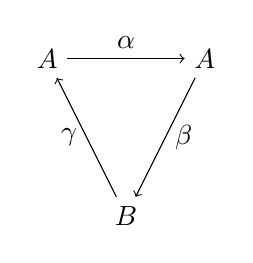
\begin{tikzpicture}
					\node (A) at (-1, 1) {$A$};
					\node (A2) at (1, 1) {$A$};
					\node (B) at (0, -1) {$B$};
					\draw[->] (A) -- node[above]{$\alpha$} (A2);
					\draw[->] (A2) -- node[right]{$\beta$} (B);
					\draw[->] (B) -- node[left]{$\gamma$} (A);
				\end{tikzpicture}
				\caption{Exact couple.}
				\label{fig:exact_couple}
			\end{subfigure}
			\begin{subfigure}{0.49\textwidth}
				\centering
				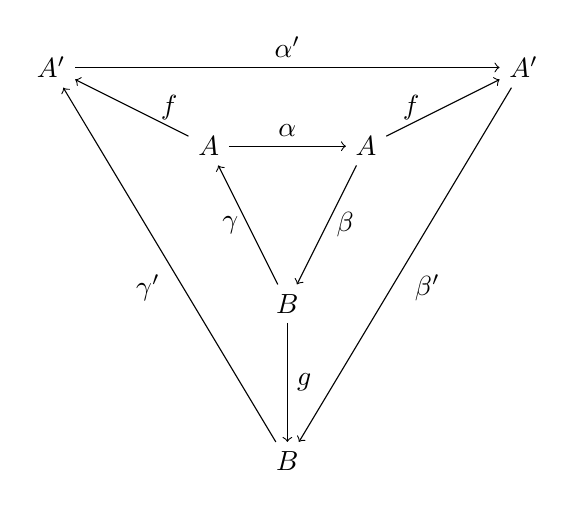
\begin{tikzpicture}
					\node (A') at (-3, 3) {$A'$};
					\node (A2') at (3, 3) {$A'$};
					\node (B) at (0, 0) {$B$};
					\node (A) at (-1, 2) {$A$};
					\node (A2) at (1, 2) {$A$};
					\node (B') at (0, -2) {$B$};
					\draw[->] (A') -- node[above]{$\alpha'$} (A2');
					\draw[->] (A2') -- node[below right]{$\beta'$} (B');
					\draw[->] (B') -- node[below left]{$\gamma'$} (A');
					\draw[->] (A) -- node[above]{$\alpha$} (A2);
					\draw[->] (A2) -- node[right]{$\beta$} (B);
					\draw[->] (B) -- node[left]{$\gamma$} (A);
					\draw[->] (A) -- node[right, xshift=7pt]{$f$} (A');
					\draw[->] (A2) -- node[left, xshift=-5pt]{$f$} (A2');
					\draw[->] (B) -- node[right]{$g$} (B');
				\end{tikzpicture}
				\caption{Morphism of exact couples.}
				\label{fig:exact_couple_morphism}
			\end{subfigure}
			\caption{Category of exact couples.}
			\label{fig:exact_couples_category}
		\end{figure}
	}
	From any exact couple $(A,B,\alpha,\beta,\gamma)$ one can construct a spectral sequence using the following prescription:
	\begin{align}
		E_0 &:= B\\
		\dr_0 &:= \beta\circ\gamma\\
		&\nonumber\\
        &\ \vdots\nonumber\\
        &\nonumber\\
		E_n &:= \frac{\gamma^{-1}(\alpha^n(A))}{\beta(\alpha^{-n}(0))}\\
		\dr_n &:= \beta\circ\alpha^{-n}\circ\gamma
	\end{align}
	It is not hard to see that $E_{n+1}=H(E_n,\dr_n)$, so this construction gives a functor from the category of exact couples to the category of spectral sequences. The higher exact couples $(\alpha^nD,E_n,\ldots)$ are sometimes called \textbf{derived couples}.

	One can also define the term $E_\infty$ using the following limit procedure. For every $n\in\mathbb{N}$, take the elements in $E_n$ that are closed under $d_n$ and call these $E_{n,n+1}$. Since there exists a canonical surjection $E_{n,n+1}\rightarrow E_{n+1}$, one can look at all the elements in $E_{n,n+1}$ for which the image in $E_{n+1}$ is closed under $d_{n+1}$. Call the set of these elements $E_{n,n+2}$. The elements that remain after taking the limit of this operation form the set $E_{n,\infty}$. Now, take the direct limit of the $E_{n,\infty}$ to obtain $E_\infty$. This is equivalent to
	\begin{gather}
		E_\infty := \frac{\cap_iZ(E_i)}{\cup_iB(E_i)},
	\end{gather}
	i.e.~$E_\infty$ contains the equivalence classes of elements that are cycles for all $d_n$ but boundaries for none. If $E_\infty$ is the associated graded object of some filtered object $G$, one says that the spectral sequence \textbf{converges} to $G$.

	Now, consider a differential object $(C,\dr)$ together with a filtration $\{F_nC\}_{n\in\mathbb{N}}$. Definition \ref{set:filtration} of a filtration immediately gives a short exact sequence for every $n\in\mathbb{N}$:
	\begin{gather}
		0\longrightarrow F_{n-1}C\longrightarrow F_nC\longrightarrow F_nC/F_{n-1}C\longrightarrow 0.
	\end{gather}
	This short sequence in turn gives rise to a long exact sequence in homology, which can be expressed as an exact triangle, and this triangle further leads to an exact couple:
	\begin{gather}
		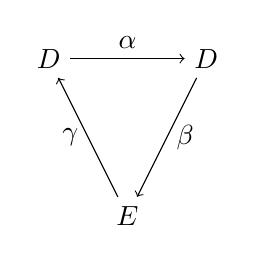
\begin{tikzpicture}
			\node (A) at (-1, 1) {$D$};
			\node (A2) at (1, 1) {$D$};
			\node (B) at (0, -1) {$E$};
			\draw[->] (A) -- node[above]{$\alpha$} (A2);
			\draw[->] (A2) -- node[right]{$\beta$} (B);
			\draw[->] (B) -- node[left]{$\gamma$} (A);
		\end{tikzpicture}
	\end{gather}
	where $D_n=H(F_nC)$ and $E_n=H(F_nC/F_{n-1}C)$. From a more abstract, yet more useful, point of view one can consider the object $E$ as a functor from the category of filtered (differential) objects to the category of graded objects. As such it is constructed from the composition of the homology functor $H$ and the ``associated graded object''-functor \[\mathrm{Gr}:C\mapsto\Big\{G_nC := F_nC/F_{n-1}C\Big\}_{n\in\mathbb{N}}\,.\]

	On the other hand, one could of course also construct the composition $\mathrm{Gr}\circ H$ that first maps a differential object to its homology object and then builds the graded object associated to the filtration \[F_nH(C):=\im\big(H(F_nC)\rightarrow H(C)\big).\] Some straightforward questions can arise at this point: ``\textit{How are the functors $H\circ\mathrm{Gr}$ and $\mathrm{Gr}\circ H$ related?}'', ``\textit{Do they coincide?}'', ... The latter question is easily answered: ``\textit{No, they do not.}'' However, they can be related and this exactly happens through a spectral sequence that says how the homology of the graded object associated to $C$ can be related to the homology of $C$ itself.

\subsection{Filtered complexes}

	For the remainder of this section only graded differential objects will be considered, i.e.~$(C_\bullet,\dr_\bullet)=(\{C_p\}_{p\in\mathbb{Z}},\dr)$ such that $\dr C_p\subseteq C_p$. In this case the exact couple consist of $D_{p,q}:=H_q(F_pC_\bullet)$ and $E_{p,q}:=H_q(G_pC_\bullet)$ and, consequently, the objects are bigraded. The filtration is also required to be compatible with the differential, i.e.~$\dr F_iC_j\subseteq F_iC_{j-1}$.

	\sremark{In contrast to most of the literature, the ``complementary convention'', i.e.~the convention where $p+q$ denotes the total degree and hence $E_{p,q}=H_{p+q}(G_pC_\bullet)$, is not adopted.}

	Before introducing an expression for a general page $E_r$, the terms of degree zero and one are considered to get some intuition. The differential on $E_0$ is given by
	\begin{gather}
		\dr_0:\frac{F_pC_q}{F_{p-1}C_q}\rightarrow\frac{F_pC_{q-1}}{F_{p-1}C_{q-1}}
	\end{gather}
	and is induced by the differential $\dr$ on $C_\bullet$. The kernel of this map is clearly given by all elements $x\in F_pC_q$ such that $\drx=0\mod F_{p-1}C_{q-1}$ (with the additional remark that one also has to take the quotient by $F_{p-1}C_q$). As a result one finds that the homology $E_1=H(E_0,\dr_0)$ is given by
	\begin{gather}
		E_1^{p,q}:=\frac{\{x\in F_pC_q\mid\drx\in F_{p-1}C_{q-1}\}}{F_{p-1}C_q+\dr F_pC_{q+1}}.
	\end{gather}
	The first term in the denominator was already explained above. The second term comes from the $\im(\dr_0)$-part in the definition of $H(E_0,\dr_0)$. One might suspect that some data is missing since the relevant map $\dr_0^{p,q+1}$ goes from $\frac{F_pC_{q+1}}{F_{p-1}C_{q+1}}$ to $\frac{F_pC_q}{F_{p-1}C_{q}}$. However, the image of $F_{p-1}C_{q+1}$ is a subspace of $F_{p-1}C_q$ and this is already included in the first term, so one might as well work with all of $F_pC_{q+1}$.

	For arbitrary $r>0$, one defines the page $E_r$ as follows:
	\begin{gather}
    	E_r^{p,q}:=\frac{\{x\in F_pC_q\mid\drx\in F_{p-r}C_{q-1}\}}{F_{p-1}C_q+\dr F_{p+r-1}C_{q+1}}.
	\end{gather}

    To relate this more to the usual notions of (co)homology, one can rephrase this in terms of (co)chains, (co)cycles and (co)boundaries. Consider again a filtered complex $F_\bullet C_\bullet$. The following definitions are used:
    \begin{itemize}
        \item The elements of $G_pC_q$ are called the $(p,q)$-\textbf{chains} (in filtering degree $p$).
        \item The elements of \[Z^r_{p,q} := \{c\in G_pC_q\mid\dr c=0\bmod F_{p-r}C_{q-1}\}\] are called $r$-\textbf{almost} $(p,q)$-\textbf{cycles}.
        \item The elements of \[B^r_{p,q} := \dr F_{p+r-1}C_{q+1}\] are called $r$-\textbf{almost} $(p,q)$-\textbf{boundaries}.
    \end{itemize}
    It is then easy to see that the page $E^r$ satisfies
    \begin{gather}
        E^r_{p,q} = Z^r_{p,q}/B^r_{p,q},
    \end{gather}
    i.e.~the homology is given by the quotient of the cycles by the boundaries. All these objects fit in a nice sequence of inclusions:
    \begin{gather}
        B^0_{p,q}\hookrightarrow\cdots\hookrightarrow B^\infty_{p,q}\hookrightarrow Z^\infty_{p,q}\hookrightarrow\cdots\hookrightarrow Z^0_{p,q}.
    \end{gather}

\subsection{Convergence}

    \newdef{Limit term}{\index{limit}
        Consider a spectral sequence $\{E^r_{p,q}\}$. If there exists a for every two integers $p,q\in\mathbb{Z}$ an integer $r(p,q)\in\mathbb{N}$ such that for all $r\geq r(p,q)$:
        \begin{gather}
            E^r_{p,q}\cong E^{r(p,q)}_{p,q}\,,
        \end{gather}
        the object $E^\infty:=\{E^{r(p,q)}_{p,q}\}$ is called the \textbf{limit term} and the sequence is said to \textbf{abut} to $E^\infty$.
    }
    \begin{example}[Collapsing sequence]
        If there exists an integer $r\in\mathbb{N}$ such that for all $s\geq r:d_s=0$, the sequence is said to \textbf{collapse} at $r$ and $E^r$ is a limit term. A common example is where the nonvanishing elements of a term are concentrated in a single row or column.
    \end{example}

    \newdef{Convergence}{\index{convergence}
        A spectral sequence ${E^r_{p,q}}$ is said to converge to a graded object $H_\bullet$ with filtering $F_\bullet H_\bullet$, denoted by \[E^r_{p,q}\Rightarrow H_\bullet\,,\] if
        \begin{gather}
            E^\infty_{p,q}\cong G_p H_q\qquad\qquad\forall p,q\in\mathbb{Z}.
        \end{gather}
    }

    \newdef{Bounded sequence}{\index{bounded!sequence}
        A spectral sequence is said to be bounded if for all numbers $n,r\in\mathbb{Z}$, there only exists a finite number of nonvanishing elements of the form $E^r_{k,n-k}$. A common example are the \textbf{first quadrant spectral sequences} where the only nonvanishing elements have $p,q\geq0$.
    }
    \begin{property}
        Every bounded spectral sequence abuts.
    \end{property}

    \begin{property}[Filtered complex]
        If the spectral sequence of a filtered complex $F_\bullet C_\bullet$, it converges to the chain homology of the complex:
        \begin{gather}
            E^r_{p,q}\Rightarrow H_\bullet(C).
        \end{gather}
    \end{property}

    ?? COMPLETE ??

\section{Examples}
\subsection{Group cohomology}\index{group!cohomology}\label{section:group_cohomology}

	In this section an important application of derived functors is given. In fact, historically this was one of the motivating applications. In different areas of mathematics and physics, the concept of group cohomology pops up. Some examples are the obstruction to group extensions, the classification of projective representations and the application of these concepts to the study of symmetry-protected topological order in condensed matter physics. However, the literature on these applications often starts with an ad hoc construction based on maps from a group to a module:
    \newdef{Group cohomology}{\label{homalg:group_cohomology}
        Consider a group $G$ together with a $G$-module $A$. (For simplicity only discrete, e.g.~finite, groups and Abelian coefficients will be considered.) For every $k\in\mathbb{N}$, define the $k^{th}$ \textbf{chain group} as
        \begin{gather}
            C^k(G;A) := \big\{\text{all set-theoretic functions from }G^k\text{ to }A\big\}.
        \end{gather}
        The coboundary map $\dr^k:C^k(G;A)\rightarrow C^{k+1}(G;A)$ is defined as follows:
        \begin{align}
            \dr^kf(g_1,\ldots,g_k,g_{k+1}) := g_1\cdot f(g_2,\ldots,&g_k,g_{k+1}) + (-1)^{k+1}f(g_1,\ldots,g_k)\nonumber\\
            &+\sum_{i=1}^k(-1)^{i+1} f(g_1,\ldots,g_ig_{i+1},\ldots,g_k,g_{k+1}).
        \end{align}
        The cohomology groups are defined as the following quotient groups:
        \begin{gather}
            H^k(G;A) := \frac{\ker(\dr^k)}{\im(\dr^k)}.
        \end{gather}
    }

    Every $G$-module \ref{group:module} can be regarded as a module over the group ring $\mathbb{Z}[G]$, i.e.~there exists an equivalence of categories between $\mathbf{Ab}$ and $\mathbb{Z}[G]\mathbf{Mod}$. Assuming the axiom of choice, every module category over a ring has enough projectives and, hence, it makes sense to define group (co)homology using derived functors in $\mathbb{Z}[G]\mathbf{Mod}$. An explicit construction of a resolution that is not just $\mathbb{Z}[G]$-projective but even $\mathbb{Z}[G]$-free will be given.

	The homology and cohomology of a finite group $G$ with coefficients in a $G$-module $A$ is defined using the Ext- and Tor-functors defined above:
	\begin{align}
		H^\bullet(G;A) &:= \mathrm{Ext}_{\mathbb{Z}[G]}^\bullet(\mathbb{Z},A)\\
		H_\bullet(G;A) &:= \mathrm{Tor}^{\mathbb{Z}[G]}_\bullet(A,\mathbb{Z})\,,
	\end{align}
	where $\mathbb{Z}$ carries the trivial $G$-module structure. To explicitly calculate the (co)homology groups, one has to find an acyclic resolution of $\mathbb{Z}$:
	\begin{construct}[Normalized bar resolution]\index{resolution!bar}
		Let $P'_k$ be a free rank-$k$ $G$-module. The boundary maps are defined as follows:
		\begin{align}
			\label{homalg:group_boundary}
			\partial_k(g_1,\ldots,g_k) = g_1(g_2,\ldots,g_k) + \sum_{i=1}^k (-1)^i(g_1,&\ldots,g_ig_{i+1},\ldots,g_k)\\
             &+ (-1)^k(g_1,\ldots,g_{k-1}).\nonumber
		\end{align}
		To obtain the normalized bar\footnote{One of the possible explanations for this name is that the formal generating elements are often written as $[g_1|g_2|\ldots|g_k]$.} resolution (in inhomogeneous form), one has to quotient out the submodule of $P'_n$ generated by tuples $(g_1,\ldots,g_n)$ where one of the $g_i$'s is the identity. It can be shown that the resulting quotient modules $P_n$ form a $\mathbb{Z}[G]$-free resolution of $\mathbb{Z}$.
	\end{construct}

	To explicitly calculate the cohomology groups $H^k(G;A) = H^k(\hom_{\mathbb{Z}[G]}(P_\bullet,A))$, it is often easier to work with a more explicit description of the involved hom-sets. Since $P_k$ is a free $\mathbb{Z}[G]$-module on $G^k$, it is isomorphic (as a module) to $\mathbb{Z}[G^{k+1}]$. This can be seen as follows. The generating set consists of all $k$-tuples of elements in $G$: \[S=\{(g_1,\ldots,g_k)\mid\forall i\leq k:g_i\in G\}.\] Since the module is free over $\mathbb{Z}[G]$, one can write every element as a formal linear combination of elements of the form \[g_0(g_1,\ldots,g_k).\] One can now construct a morphism $\varphi$ between this module and $\mathbb{Z}[G^{k+1}]$, which carries the diagonal $G$-action, in the following way. On the generating set $S$, define $\varphi$ as follows:
	\begin{gather}
		\varphi(g_1,\ldots,g_k) := (e,g_1,g_1g_2,\ldots,g_1g_2\cdots g_k).
	\end{gather}
	It is not hard to show that this morphism is in fact an isomorphism (of $G$-modules) and that
	\begin{gather}
		H^k(G;A) = H^k(\hom_{\mathbb{Z}[G]}(\mathbb{Z}[G^{k+1}],A)).
	\end{gather}
	By a little more algebra, it can also be shown that this hom-set is isomorphic to the (set-theoretic) mapping space $\mathrm{Map}(G^k,A)$. This space can be given an Abelian group structure induced by the group structure on $A$. Combining these facts, one gets the following construction for the cohomology of groups:
	\begin{construct}[Group cohomology]
		Let $G$ be a finite group and let $A$ be a $G$-module. Denote by $C^k$ the free Abelian group generated by the set-theoretic functions $f:G^k\rightarrow A$ with the property that if any of their arguments is the identity, the result is 0. The boundary maps $\partial^k$, induced by the maps defined in Equation \eqref{homalg:group_boundary}, are given by:
		\begin{align}
			(\partial^k f)(g_1,\ldots,g_{k+1}) = g_1\cdot f(g_2,\ldots,g_{k+1}) + \sum_{i=1}^k(-1)^i&f(\ldots,g_ig_{i+1},\ldots)\\
            &+(-1)^{k+1}f(g_1,\ldots,g_k).\nonumber
		\end{align}
		This is exactly the relation used to obtain group cohomology in Definition \ref{group:cohomology}.
	\end{construct}

	\begin{property}[Finiteness]
		Let $G$ be a finite group and let $A$ be a $G$-module such that the underlying group is finitely generated. Since in this case the hom-groups are themselves finitely generated, the cohomology groups $H^k(G;A)$ for $k\geq1$ are also finitely generated. Furthermore, they are annihilated by the order of $G$, so in particular they are all torsion. It follows that all cohomology groups are finite.
	\end{property}

    \begin{property}[Bockstein homomorphism]\index{Bockstein homomorphism}
        Let $G$ be a group and consider a short exact sequence of $\mathbb{Z}[G]$-modules \[0\longrightarrow A\longrightarrow B\longrightarrow C\longrightarrow0.\] This exact sequence induces a long exact sequence in group cohomology. The connecting homomorphism
        \begin{gather}
            H^\bullet(G;C)\rightarrow H^{\bullet+1}(G;A)
        \end{gather}
        is called the Bockstein homomorphism.
    \end{property}

    ?? COMPLETE (ADD e.g. classification of extensions) ??

\subsection{\difficult{Hochschild and cyclic homology}}\index{homology!Hochschild}

    \newdef{Hochschild homology groups}{\label{algebra:hochschild_homology}
        Let $A$ be an associative algebra and consider an $A$-bimodule $M$. For all $k\in\mathbb{N}$ define
        \begin{gather}
            HC_k(A;M) := M\otimes A^{\otimes k}.
        \end{gather}
        The boundary operator $\dr_k:HC_k(A;M)\rightarrow HC_{k-1}(A;M)$ is defined as follows:
        \begin{align}
            \dr_k:m\otimes a_1\otimes\cdots\otimes a_k\mapsto ma_1\otimes\cdots\otimes a_k + \sum_{i=1}^{k-1}(-1)^im\otimes a_1&\otimes\cdots\otimes a_ia_{i+1}\otimes\cdots\otimes a_k\\
            &+(-1)^ka_1m\otimes\cdots\otimes a_k.\nonumber
        \end{align}
        The Hochschild homology is then given by the homology of this chain complex:
        \begin{gather}
            H\!H_k(A;M) := \ker(\dr_k)/\im(\dr_{k+1}).
        \end{gather}
        This complex can be turned into a graded-commutative algebra by equipping it with the \textit{shuffle product}.
    }
    \begin{remark}[Cohomology]
        Hochschild cohomology of $A$ can be obtained by dualizing: $HC^k(A):=\hom\big(HC_k(A),K\big)$, where $K$ is the field over which $A$ is defined.
    \end{remark}

    \newdef{Cyclic homology}{\index{cohomology!cyclic}
        The cyclic chain complex $CC_\bullet(A)$ is the subcomplex of the Hochschild complex $HC_\bullet(A)$ obtained as the kernel of $1-\lambda$, where $\lambda$ is the permutation operator
        \begin{gather}
            \lambda:HC_k(A)\rightarrow HC_k(A):a_0\otimes\cdots\otimes a_k\mapsto(-1)^ka_k\otimes a_0\otimes\cdots\otimes a_{k-1}.
        \end{gather}
        It can be shown that the Hochschild boundary operator commutes with the permutation operator and, hence, descends to the cyclic complex. The resulting homology is called cyclic homology $CH_\bullet(A)$. As usual, by dualizing one obtains cyclic cohomology.
    }

    \begin{theorem}[Hochschild-Kostant-Rosenberg]\index{Hochschild-Kostant-Rosenberg}
        Let $A=C^\infty(M)$, where $M$ is a smooth manifold (Definition \ref{diff:manifold}).
        \begin{gather}
            H\!H_\bullet(A)\cong\Omega^\bullet(M).
        \end{gather}
    \end{theorem}

    \begin{example}[Smooth algebras]
        Consider the case of $A=C^\infty(M)$, where $M$ is a smooth manifold.
        \begin{gather}
            CH_k(A)\cong Z^k_\text{dR}(M)\oplus\bigoplus_{\substack{i=1\\k-2i\geq0}}H^{k-2i}_\text{dR}(M).
        \end{gather}
        For this reason cyclic cohomology will be used in \textit{noncommutative geometry} to generalize de Rham cohomology.
    \end{example}